\documentclass[11pt]{article}
\usepackage[margin=1in]{geometry}
\usepackage{amsmath,amssymb,bm}
\usepackage{graphicx}
\usepackage{setspace}
\usepackage{natbib}
\usepackage[hidelinks]{hyperref}

\newcommand{\by}{\mathbf{y}}
\newcommand{\bx}{\mathbf{x}}
\newcommand{\bb}{\mathbf{b}}
\newcommand{\bX}{\mathbf{X}}
\newcommand{\bP}{\mathbf{P}}
\newcommand{\bQ}{\mathbf{Q}}
\newcommand{\bK}{\mathbf{K}}
\newcommand{\bD}{\mathbf{D}}
\newcommand{\bS}{\mathbf{S}}
\newcommand{\bI}{\mathbf{I}}
\newcommand{\bA}{\mathbf{A}}
\newcommand{\blambda}{\bm{\lambda}}
\newcommand{\btau}{\bm{\tau}}
\newcommand{\bbeta}{\bm{\beta}}
\newcommand{\bzero}{\mathbf{0}}
\newcommand{\N}{\mathrm{N}}
\newcommand{\tr}{\mathrm{tr}}
\newcommand{\M}[1]{\mathcal{M}_{#1}}
\newcommand{\scen}[1]{\textsc{#1}}

\title{Bayesian adaptive distributed lag models}
\author{Alastair Rushworth}
\date{First version: January 2018 (arXiv:1801.06670v1). This revision: \today}

\begin{document}
\maketitle

\begin{abstract}
Distributed lag models (DLMs) express the cumulative and delayed dependence
between pairs of time-indexed response and explanatory variables. In practical
application, users of DLMs examine the estimated influence of a series of
lagged covariates to assess patterns of dependence. Much recent methodological
work has sought to develop flexible parameterisations for smoothing the
associated lag parameters that avoid overfitting. However, this paper finds
that some widely-used DLMs introduce bias in the estimated lag influence, and
are sensitive to the maximum lag which is typically chosen in advance of model
fitting. Simulations show that bias and misspecification are dramatically
reduced by generalising the smoothing model to allow varying penalisation of
the lag influence estimates. The resulting model is shown to have substantially
fewer effective parameters and lower bias, providing the user with confidence
that the estimates are robust to prior model choice.

\medskip\noindent
\textit{Keywords:} Distributed lag model; penalized spline; adaptive smoothing
\end{abstract}

\doublespacing

\section{Introduction}
\label{sec:intro}

Distributed lag models (DLMs) find application whenever the influence of a
time-indexed independent variable is delayed and spread over time. Although
DLMs are widely applicable, their development was originally motivated by
problems in econometrics \citep{nerlove1958, almon1965, zellner1970, haugh1977}
and they have more recently experienced a surge in popularity in environmental
epidemiology \citep{zanobetti2000, welty2009, gasparrini2010}. Crucially, DLMs
enable direct interpretation of the influence of a temporal exposure ensemble,
which is particularly useful for characterising the total health impact of
persistent environmental exposures such as air pollution or temperature
\citep{wyzga1978, gasparrini2010}. Lag models can help to identify subtle types
of time-dependence such as `mortality displacement', which occurs when exposure
related mortality diminishes a vulnerable subpopulation, resulting in lower
mortality in subsequent time intervals. Mortality displacement has been widely
documented \citep{schwartz2000, braga2001} and is conspicuous where lag
influence is estimated to have a protective effect at low or moderate lags for
what are otherwise harmful exposures \citep{zanobetti2000}. Correctly
identifying these effects depends on obtaining unbiased estimates of the
underlying lag influence, and it is therefore essential that the DLM is
correctly specified. Since no previous study has formally quantified the
estimation cost of model misspecification, this paper provides a comparison of
various existing techniques.

If a time-varying explanatory variable $X_t$ has some influence on a response
variable $Y_t$ over a set of lags $0, \ldots, p$, then a simple DLM can be
expressed as the regression model $Y_t = \sum_{i=0}^{p} X_{t-i} \beta_i +
\epsilon$, where $\epsilon$ is an independent error process and the parameters
$\bbeta = (\beta_0, \beta_1, \ldots, \beta_p)$ are referred to as the `lag
curve' or lag function, as a function of $i$. $\bbeta$ cannot be reliably
estimated using ordinary generalised linear models when $X_t$ and $X_{t-1}$ are
correlated, and regularisation using shape constraints or smoothness
restrictions over the lag parameters $\bbeta$ are frequently used. Recent
studies have implemented various forms of flexible parameterisation using
polynomial splines and smoothness penalties, for example by combining uniformly
spaced B-splines with ridge penalisation \citep{zanobetti2000},
logarithmically spaced B-splines \citep{gasparrini2010}, penalised B-splines
\citep{rushworth2013, obermeier2015}, and Bayesian penalised splines with
varying ridge penalties \citep{muggeo2008}. Spline basis representations ensure
a minimum level of smoothness, and offer computational relief when there are
fewer knots than lags, which reduces the total number of parameters to
estimate. Although smoothness restrictions primarily serve to stabilise the
model, they can also be exploited to incorporate additional structure over the
shape of the estimated lag curve. For example, it is widely assumed that the
true lag curve has more curvature at short lags than at large lags, reflecting
the intuition that recent events are generally the most influential, and
influence should decay rapidly to zero for increasing lags. Further structure
can also be used to avoid discontinuity between the influence of the final
modelled lag $\beta_p \neq 0$ and the implicitly assumed $\beta_{p+j} = 0$.
Some examples include \citet{koyck1954} who restricted $\bbeta$ to decay
geometrically with increasing $p$; \citet{muggeo2008} who combined a B-spline
basis with parameters which were shrunk by a lag-varying ridge penalty;
\citet{gasparrini2010} used logarithmic knot placement in the lag dimension to
enable varying smoothness; and \citet{welty2009} constructed a Gaussian process
prior distribution that enforces smaller covariances on lag parameters at short
lags than longer ones. While each of these approaches achieves a level of
lag-varying smoothness, each incorporates a parametric assumption on the type
of penalisation that occurs, which may not be appropriate in general.

A further problem arises because the maximum lag $p$ must be chosen before
model fitting: this is sometimes justified by drawing on previously published
studies, for example, in several studies of the delayed effects of temperature
on human health, $20 \leq p \leq 30$ is consistently reported
\citep{braga2002, armstrong2006, gasparrini2013}. In general, there is a cost
to getting $p$ wrong: too large and the model risks overfitting, and too small
can bias the resulting lag function estimate. Few studies have investigated
sensitivity of different models to choices of $p$, although several authors
recognise that this is an ongoing difficulty for DLMs. \citet{heaton2012} and
\citet{heaton2014} provide notable exceptions, and estimate $p$ as part of a
two-stage approach. However, DLMs are often applied in settings where the true
lag curve is believed to decay gradually to 0, and in such settings, $p$ is
likely to be poorly estimated and will lack a meaningful interpretation.

This paper proposes a pragmatic strategy that ensures flexible and automatic
smoothing over the lag structure that avoids the need to either estimate or
choose $p$ in advance. By exploiting the property that very large lags have
close to 0 influence, an automatic lag-dependent smoother is constructed that
ensures strong penalisation at high lags so that $p$ can be made arbitrarily
large without the risk of overfitting. This follows the tradition of richly
specifying a hierarchical model and ensuring parsimony by liberal use of
regularisation and smoothing. A new DLM is described in Section
\ref{sec:model} and in Section \ref{sec:sim} a comprehensive simulation study
illustrates the DLM's desirable properties, especially in comparison to
existing approaches. This study compares bias resulting from getting $p$
wrong, which is itself a central contribution, as DLMs have not previously
been compared in this manner. Section \ref{sec:real} applies the model
to four real data sets: daily stock market returns, intraday order flow and
prices at one-second resolution, air pollution and mortality in Chicago, and
COVID-19 cases and deaths.
Section \ref{sec:discussion} concludes the paper with an overview of the main
findings and a discussion of the implications for users of distributed lag
models.

\section{Adaptive distributed lag models}
\label{sec:model}

Define $\by = (y_1, \ldots, y_n)$, a response variable time series of length
$n$, and $\bx = (x_1, \ldots, x_n)$, a time series of an exposure or input,
whose influence on $\by$ up to some lag $p$ is to be estimated. A Gaussian DLM
for these data can be written as $y_i \sim \N\left(\sum_{j=0}^{p} x_{i-j}
\beta_j,\ \sigma^2\right)$ where $i = p+1, p+2, \ldots, n$, and $\sigma^2$ is
the error variance. The lag parameters $(\beta_0, \beta_1, \ldots, \beta_p)$
could be penalised and estimated directly, but for ease of comparison with
existing approaches, these will be projected onto a B-spline basis of $K$
functions uniformly spaced over the lag range $0, \ldots, p$. The basis
representation can be expressed as $\beta_j = \sum_{k=1}^{K} B_k(j) b_k$ where
the further set of parameters $\bb = (b_1, \ldots, b_K)$ determine the fitted
lag curve. The model can be expressed as $\by \sim \N(\bX \bb,\ \sigma^2
\bI)$, where $\bX_{ik} = \sum_{j=0}^{p} x_{i-j} B_k(j)$. To control the
roughness of $b_k$ in a way that enables variable smoothing, a similar
approach to \citet{brewer2007} and \citet{reich2008} is used, in which the
intrinsic autoregressive (ICAR) prior distribution of \citet{besag1991} is
generalised. The conditional prior distribution for $\bb$ under the ordinary
ICAR is $\bb \sim \N(\bzero, \frac{1}{\lambda} \bP^{-})$, resulting in a
conditional prior density of
\begin{equation}
\pi(\bb \mid \lambda) \propto \exp\left(-\frac{\lambda}{2} \bb^\top \bP \bb\right)
= \exp\left(-\frac{1}{2} \sum_{k=1}^{K-1} \lambda (b_{k+1} - b_k)^2\right).
\label{eq:icar}
\end{equation}
The precision parameter $\lambda$ controls the extent to which the squared
differences of consecutive pairs of $\bb$ influence the posterior, imparting a
smoothing effect over the lag curve derived from $\bb$. Since each squared
difference $(b_{k+1} - b_k)^2$ contributes equally in the prior in Equation
\eqref{eq:icar}, variable smoothing can be achieved naturally by introducing a
set of precision parameters $\blambda = (\lambda_1, \ldots, \lambda_{K-1})$
that enables pairs of B-spline parameters to be smoothed more or less
strongly. This generalised prior can be written $\pi(\bb \mid \blambda)
\propto \exp\left(-\frac{1}{2} \sum_{k=1}^{K-1} \lambda_k (b_{k+1} -
b_k)^2\right) = \N(\bzero, \bQ^{-})$ where $\bQ = \bD^\top \mathrm{diag}
(\blambda) \bD$, with $\bD$ the $(K-1) \times K$ first-difference matrix, is
the precision matrix
\begin{equation*}
\bQ =
\begin{pmatrix}
\lambda_1 & -\lambda_1 & 0 & 0 & \ldots & 0 \\
-\lambda_1 & \lambda_1 + \lambda_2 & -\lambda_2 & 0 & \ldots & 0 \\
0 & -\lambda_2 & \lambda_2 + \lambda_3 & -\lambda_3 & \ldots & 0 \\
\vdots & \vdots & \vdots & \vdots & \ddots & \vdots \\
0 & 0 & 0 & 0 & -\lambda_{K-1} & \lambda_{K-1}
\end{pmatrix}.
\end{equation*}
$\bQ$ has rank $K - 1$ and its null space is spanned by the constant vector,
so the prior is intrinsic: it is improper with respect to the overall level of
$\bb$ but proper for the differences, and $\bQ^{-}$ denotes a generalised
inverse. The posterior distribution is nevertheless proper, since the level of
$\bb$ is identified by the likelihood. This joint specification for $\bb$
results in the conditional distributions
\begin{equation*}
b_k \mid \bb_{-k}, \blambda \sim
\begin{cases}
\N\left(b_{k+1},\ \frac{1}{\lambda_1}\right) & \text{if } k = 1 \\[6pt]
\N\left(\frac{\lambda_{k-1} b_{k-1} + \lambda_k b_{k+1}}{\lambda_{k-1} + \lambda_k},\
\frac{1}{\lambda_{k-1} + \lambda_k}\right) & \text{if } k = 2, \ldots, K-1 \\[6pt]
\N\left(b_{k-1},\ \frac{1}{\lambda_{K-1}}\right) & \text{if } k = K.
\end{cases}
\end{equation*}
When $\lambda_1 = \lambda_2 = \ldots = \lambda_{K-1} = \lambda$, then $\bQ =
\lambda \bP$, which shows that the ordinary ICAR prior in Equation
\eqref{eq:icar} is a special case of the adaptive prior.

The influence of very large lags is expected to be negligible, and a lag
curve that terminates away from zero at lag $p$ would imply an artificial
discontinuity with the implicitly assumed $\beta_{p+j} = 0$. Rather than
modifying $\bQ$, this is discouraged by a single pseudo-observation: the row
$(B_1(p), \ldots, B_K(p))$ is appended to $\bX$ together with a zero response,
which contributes the factor $\exp\{-\beta_p^2 / (2\sigma^2)\}$ to the
posterior and so shrinks the final value of the lag curve towards zero at the
scale of the error variance, without introducing an additional tuning
parameter. Alternatively the constraint $\beta_p = 0$, optionally together with
$\beta'_p = 0$, can be imposed exactly by restricting $\bb$ to the null space
of the constraint rows, which leaves the generalised determinant above
unchanged up to a constant; this is the default in the accompanying software.

A further smoothing prior distribution is placed over $\blambda$ to restrict
their flexibility. This is particularly attractive as it also reflects our
intuition that the curvature of the lag function should not change too
rapidly. For this purpose, an ordinary ICAR prior is used to smooth the log
precisions $\btau = (\tau_1, \ldots, \tau_{K-1})$, $\tau_k = \log
\lambda_k$, such that $\btau \mid \zeta^2 \sim \N(\bzero, \zeta^2 \bK^{-})$
where $\bK$ is the $(K-1) \times (K-1)$ precision matrix
\begin{equation*}
\bK =
\begin{pmatrix}
1 & -1 & 0 & 0 & \ldots & 0 \\
-1 & 2 & -1 & 0 & \ldots & 0 \\
0 & -1 & 2 & -1 & \ldots & 0 \\
\vdots & \vdots & \vdots & \vdots & \ddots & \vdots \\
0 & 0 & 0 & 0 & \ldots & 1
\end{pmatrix}.
\end{equation*}
Therefore, for small values of the variance $\zeta^2$, pairs of consecutive
elements of $\btau$ are more strongly smoothed towards each other. Finally,
the variance parameters were assigned weakly informative inverse-gamma priors,
$\sigma^2 \sim \mathrm{IG}(0.001, 0.001)$ and $\zeta^2 \sim \mathrm{IG}(1,
1/2)$, the values used in the accompanying R package. The combination of
adaptive smoothing with smoothed variances as described results in a very
flexible model that can accommodate complex shapes using a relatively simple
specification. The model described above assumes Gaussian errors for
simplicity, but the ideas easily generalise to accommodate other response
distributions.

Inference for the models fitted in the simulation study in Section
\ref{sec:sim} was achieved using Markov chain Monte Carlo (MCMC) simulation
using a mixture of Gibbs sampling and Metropolis--Hastings steps, implemented
in R \citep{rcore2016}. The accompanying software, the Python package
\texttt{badlm} (\url{https://github.com/alastairrushworth/badlm}), uses a
different scheme that is considerably more efficient. Given $\btau$ and
$\sigma^2$ the model is linear and Gaussian, so $\bb$ can be integrated out
analytically: with $\bA = \bQ + \bX^\top \bX / \sigma^2$ and $\mathbf{m} =
\bX^\top \by / \sigma^2$,
\begin{equation*}
\log p(\by \mid \btau, \sigma^2) = -\frac{n}{2} \log (2\pi\sigma^2)
+ \frac{1}{2} \log |\bQ|_{+} - \frac{1}{2} \log |\bA|
+ \frac{1}{2} \mathbf{m}^\top \bA^{-1} \mathbf{m}
- \frac{\by^\top \by}{2\sigma^2},
\end{equation*}
where $|\bQ|_{+}$ is the generalised determinant of the intrinsic prior
precision, the product of its non-zero eigenvalues. Since the pairs $(b_k,
b_{k+1})$ penalised by $\bQ$ form a chain, the matrix-tree theorem gives
$|\bQ|_{+} = K \prod_{k=1}^{K-1} \lambda_k$, so this term is simply $\log K +
\sum_k \tau_k$. The resulting marginal posterior of $(\btau, \sigma^2)$ is
smooth and low dimensional, and is sampled with the No-U-Turn Sampler
\citep{hoffman2014} using automatic differentiation; $\bb$ is then drawn from
its Gaussian conditional distribution for each retained draw. Collapsing
removes the strong dependence between $\bb$ and $\btau$ that slows a Gibbs
sampler, and each likelihood evaluation costs $O(K^3)$ regardless of $n$
because only the sufficient statistics $\bX^\top \bX$ and $\bX^\top \by$ are
needed. The software also provides a Gibbs sampler with slice updates of
$\btau$ as an independent check, a Laplace approximation to the collapsed
posterior that serves as a fast approximate fit and as the starting point of
the chains, an exact version of the end constraint, AR(1) errors and
Poisson and negative binomial responses.

\section{Simulation study}
\label{sec:sim}

The adaptive model detailed in Section \ref{sec:model} was compared with
several currently available distributed lag models, labelled $\M{1}$, $\M{2}$,
$\M{3}$, $\M{4}$ and $\M{5}$. $\M{1}$ is a non-adaptive version of the DLM
described in Section \ref{sec:model} (achieved by fixing $\lambda_1 = \lambda_2
= \ldots = \lambda_{K-1} = \lambda$), $\M{2}$ is a Bayesian implementation of
the DLM with linearly increasing ridge penalty proposed by \citet{muggeo2008},
$\M{3}$ is the new adaptive model described in Section \ref{sec:model},
$\M{4}$ is the P-spline model of \citet{obermeier2015} and $\M{5}$ is the DLM
with logarithmically spaced knots of \citet{gasparrini2010}.

\subsection{Comparison under different lag structures}
\label{sec:sim1}

To compare estimation performance of models $\M{1}$--$\M{5}$, time series
response and covariate data were simulated assuming each of five
different-shaped lag relationships, each with maximum lag $p = 50$. The curves
are shown in Figure \ref{fig:curves} and included a delayed peak scenario
(\scen{Delayed peak}), an exponential decay curve (\scen{Decay curve}), a
horizontal line at 0 equivalent to a null effect (\scen{Flat response}), a
curve exhibiting a shape similar to a mortality displacement effect
(\scen{Displacement}) and a sharply peaked function that declines rapidly to
0 (\scen{Sharp peak}).

A covariate time series, $x_t$, was generated by assuming $x_t \sim \N(0.5
x_{t-1}, 0.1^2)$, and conditional on each lag function, a response series
$y_t$ was generated using $y_t = \sum_{j=0}^{50} \beta_j x_{t-j} +
\epsilon_t$ for $t = 51, \ldots, 500$. The error term $\epsilon_t$ assumed
autocorrelation such that $\epsilon_t \sim \N(0.2 \epsilon_{t-1}, 0.1^2)$,
whose parameters were selected for an acceptable signal-to-noise ratio. The
autocorrelation in both $x_t$ and $\epsilon_t$ reflects the temporal
dependence in covariates and errors typically observed in real data.

\begin{figure}[t]
\centering
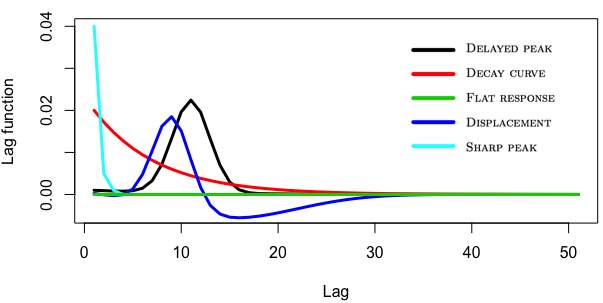
\includegraphics[width=0.85\textwidth]{figures/fig1_lag_curves.png}
\caption{The five lag curves used to simulate response and covariate data
with different lag response.}
\label{fig:curves}
\end{figure}

Models $\M{1}$--$\M{5}$ were fitted to each of 200 realisations of the
processes $\{x_t, y_t\}$ described above. The models were assessed in terms of
their ability to recover the true lag curve, as measured by root-mean squared
error (RMSE) and squared bias (Bias$^2$) of the estimates, defined for the
$j$th simulation as $\left(\frac{1}{51} \sum_{i=0}^{50} (\hat{\beta}_i^{(j)}
- \beta_i^{(j)})^2\right)^{1/2}$ and $\left(\frac{1}{51} \sum_{i=0}^{50}
\hat{\beta}_i^{(j)} - \beta_i^{(j)}\right)^2$, respectively. Following
\citet{hodges2001}, model complexity was recorded for fitted model
$\M{i}^{(j)}$ using the effective degrees of freedom $\mathrm{ED} =
\tr[\bX(\bX^\top \bX + \hat{\bS}_{\M{i}^{(j)}})^{-1} \bX^\top]$ where
$\hat{\bS}_{\M{i}^{(j)}}$ is the estimated penalty component for the $i$th
model fitted to the $j$th simulation. In particular, $\hat{\bS}_{\M{1}^{(j)}}
= \hat{\lambda}^{(j)} \mathrm{diag}(1, 2, \ldots, p+1)$;
$\hat{\bS}_{\M{2}^{(j)}} = \hat{\lambda}^{(j)} \bP$; $\hat{\bS}_{\M{3}^{(j)}}
= \hat{\bQ}^{(j)}$ and $\hat{\bS}_{\M{4}^{(j)}} = \hat{\lambda}^{(j)} \bP +
\hat{\rho}^{(j)} \bI$. For models $\M{1}$--$\M{4}$ the model matrix $\bX$ was
identical, resulting from assuming $(2/3) \times (p + 1) = 34$ uniformly
spaced B-spline basis functions to represent the lag curve, such that the
$(i,k)$th element, $\bX_{i,k} = \sum_{j=0}^{p} x_{i-j} B_k(j)$. Since lag curve
smoothness for $\M{5}$ is decided by finding the number of logarithmically
spaced knots that minimises AIC, the effective dimension in this case is the
number of knots, $\mathrm{ED} = n_z^{(j)}$ for the $j$th simulation.

\begin{table}[t]
\centering
\begin{tabular}{llrrrrr}
\hline
Lag curve shape & Summary & $\M{1}$ & $\M{2}$ & $\M{3}$ & $\M{4}$ & $\M{5}$ \\
\hline
 & RMSE & 17.31 & 14.53 & 10.32 & 15.51 & 22.68 \\
\scen{Delayed peak} & Bias$^2$ & 3.31 & 3.24 & 3.32 & 9.59 & 3.83 \\
 & ED & 18.53 & 14.99 & 7.12 & 12.14 & 15.81 \\
\hline
 & RMSE & 16.57 & 11.59 & 8.45 & 9.46 & 14.15 \\
\scen{Decay curve} & Bias$^2$ & 1.45 & 1.65 & 2.32 & 4.30 & 0.79 \\
 & ED & 18.15 & 11.54 & 5.42 & 6.40 & 7.88 \\
\hline
 & RMSE & 16.60 & 8.80 & 1.59 & 2.00 & 13.68 \\
\scen{Flat response} & Bias$^2$ & 1.14 & 0.82 & 0.28 & 0.22 & 1.51 \\
 & ED & 18.07 & 8.08 & 0.77 & 0.68 & 7.74 \\
\hline
 & RMSE & 17.32 & 14.13 & 11.24 & 15.29 & 20.34 \\
\scen{Displacement} & Bias$^2$ & 2.79 & 3.30 & 3.36 & 8.79 & 2.51 \\
 & ED & 18.55 & 13.97 & 7.97 & 12.78 & 13.37 \\
\hline
 & RMSE & 23.98 & 16.65 & 10.97 & 27.72 & 14.07 \\
\scen{Sharp peak} & Bias$^2$ & 16.01 & 11.63 & 6.81 & 24.45 & 0.86 \\
 & ED & 19.09 & 11.05 & 3.86 & 10.85 & 7.94 \\
\hline
\end{tabular}
\caption{Estimated lag function RMSE, squared bias and effective degrees of
freedom for five different types of lag curve shape, averaged across 200
simulated data sets. RMSE and Bias$^2$ have each been scaled by $10^3$.}
\label{tab:sim}
\end{table}

Table \ref{tab:sim} shows the average RMSE, Bias$^2$ and ED for each model
and lag curve scenario combination. The adaptive model, $\M{3}$, outperformed
all of the models in terms of RMSE across all lag curve scenarios. Large
separations were observed in model complexity across each scenario, with the
adaptive smoothing $\M{3}$ resulting in the lowest ED across all non-null
scenarios, ranging between 3.86 to 7.97 compared to 6.4 and 19.09 for the
other models. A particularly concerning result is that only $\M{3}$ and
$\M{4}$ correctly result in degrees of freedom $\approx 1$ under the
\scen{Flat response} scenario, compared to a range of 7.7 and 18 for the
others, which suggests that other approaches may falsely identify structure
when none exists at all. Bias was generally low across all models and
scenarios, although higher values were noted across $\M{1}$--$\M{4}$ under the
\scen{Sharp peak} scenario. As might be expected, the log-spaced knots of
$\M{5}$ performed favourably when lag influence declined rapidly from 0
(\scen{Sharp peak}), and much less so when the strongest lag effect was larger
than 0 (\scen{Delayed peak}, \scen{Displacement}). The comparison clearly
highlighted the need for care in choosing a lag smoother in practical
application, and that the quality of fit strongly depends on the underlying
lag function. Furthermore, the simulations provide encouraging evidence that
the newly proposed adaptive model is far more robust to these underlying
differences, and might be a suitable choice when little is known about the
structure being estimated.

\subsection{DLM misspecification with maximum lag $p$}
\label{sec:sim2}

Next, simulation was used to explore robustness of $\M{1}$--$\M{5}$ to
different choices of maximum lag $p$. The series $x_t$ and $y_t$ were
generated exactly as in Section \ref{sec:sim1}, using only the
\scen{Displacement} lag function with 50 lags. The models $\M{1}$--$\M{5}$
were fitted to the simulated $x_t$ and $y_t$, assuming maximum lags of $p =
50, 75, 100, 125$. To ensure the fairest comparison, the range of flexibility
for each model was restricted so that $0 < \mathrm{ED} < 2p/3$, and also
ensured that lag curve flexibility could grow proportionally with $p$. For
each of 200 fits, the RMSE of the lag curve estimate, ED and squared bias were
recorded and the results are summarised in Figure \ref{fig:ed}.

\begin{figure}[t]
\centering
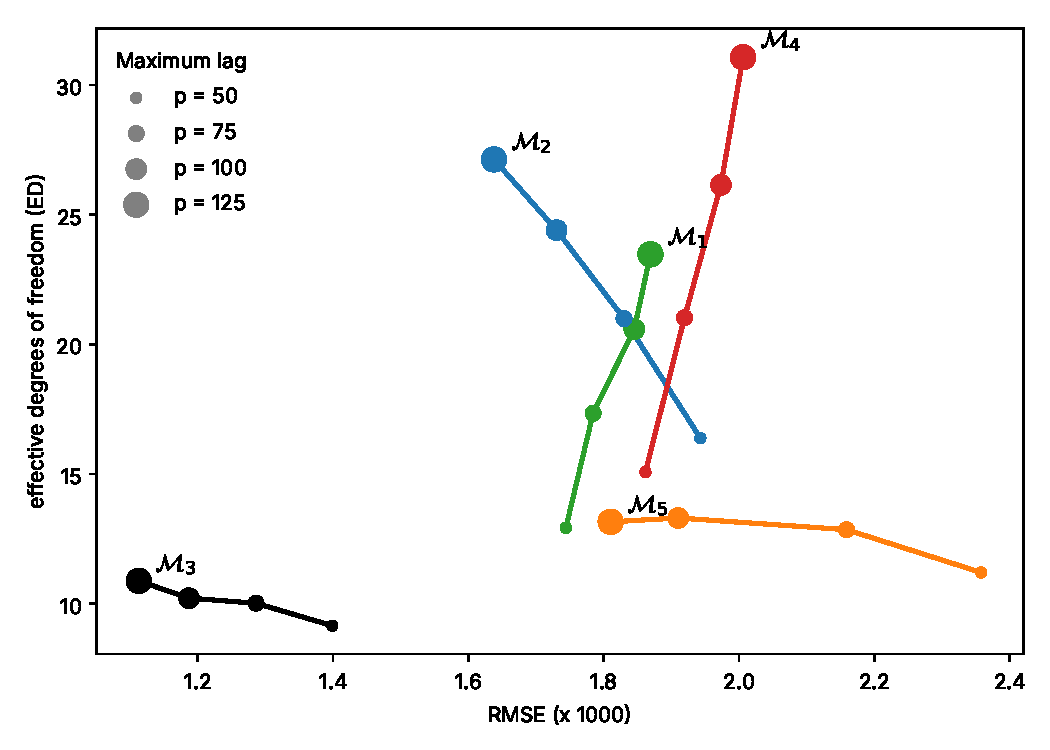
\includegraphics[width=0.7\textwidth]{figures/fig2_ed_rmse.pdf}
\caption{Effective number of parameters and RMSE for each of
$\M{1}$--$\M{5}$. Increasing diameter of the plotting symbols indicates larger
numbers of maximum lags assumed in advance of model fitting.}
\label{fig:ed}
\end{figure}

Figure \ref{fig:ed} clearly illustrates, for $\M{1}$ and $\M{5}$, that ED
increases steeply with $p$, even though the underlying true lag function is
identical. Furthermore, both the RMSE and ED are substantially smaller for the
adaptive model $\M{3}$ compared to any of the others in the comparison, and
indicate much better overall performance. The new adaptive approach $\M{3}$
is more robust to user misspecification of `large' $p$, and the simulations
raise concerns about the potential for overfitting using existing approaches.
However, it is noted that the effective degrees of freedom for $\M{3}$ are
not constant and do increase modestly with $p$, from 6.7 ($p = 50$) to 7.4
($p = 125$). Model $\M{2}$ resulted in a comparatively favourable balance
between RMSE and degrees of freedom, reinforcing the suggestion that adaptive
models are preferable choices.

\section{Illustrations with real data}
\label{sec:real}

Four applications illustrate how the adaptive lag curve behaves on noisy real
data. Both use the accompanying software with its default settings: the random
walk prior on the log precisions, an exact zero constraint at the maximum lag,
$K = \lceil 2(p+1)/3 \rceil$ basis functions, and the collapsed NUTS sampler
with two chains of 1000 retained draws. Effective degrees of freedom are
reported for the lag curve alone, excluding unpenalised terms. The scripts
that reproduce them are in the software repository.

\subsection{Daily stock market data}

Prices are not stationary, so they are transformed to percentage log returns
$r_t = 100 \log(P_t / P_{t-1})$. Daily closing prices of the S\&P 500 index and
of Apple, and closing values of the VIX implied volatility index, were obtained
for 2007 to 2016, 2,306 trading days spanning the 2008 crisis. Figure
\ref{fig:stocks} shows four lag curves. Panels (a) and (b) regress the next
day's return on the preceding 20 days' returns, the linear information that a
trading rule could exploit. For the index the curve is negative at lag one,
$-0.10$ (95\% interval $-0.15$ to $-0.06$) per percentage point, and returns to zero within a week: a short-lived
reversal with cumulative effect $-0.23$ ($-0.42$ to $-0.03$) and 4.7 effective degrees of freedom.
For Apple the curve is indistinguishable from zero at every lag, with 1.7
effective degrees of freedom; the adaptive smoother reports an absence of
structure rather than inventing it. Panel (c) regresses the daily change in
log VIX on the same day's and the preceding 60 days' index returns. The
contemporaneous coefficient is $-4.1$ ($-4.2$ to $-3.9$), so implied volatility rises about
4 per cent for each percentage point the index falls; it is followed
by a small positive rebound over the following week as the shock partly
reverses, and by nothing beyond about ten days. Panel (d) regresses the log
absolute return, a measure of realised volatility, on its own past over 100
days. The curve is strongest at lags two to three, decays over about a month
and remains small but mostly positive thereafter, the long memory of
volatility; the cumulative elasticity is 0.84 (0.75 to 0.94) and the smoother
describes 100 lags with 7.9 effective degrees of freedom. In each panel the band widens where the data are least informative
and the curve is pinned to zero at the maximum lag.

\begin{figure}[t]
\centering
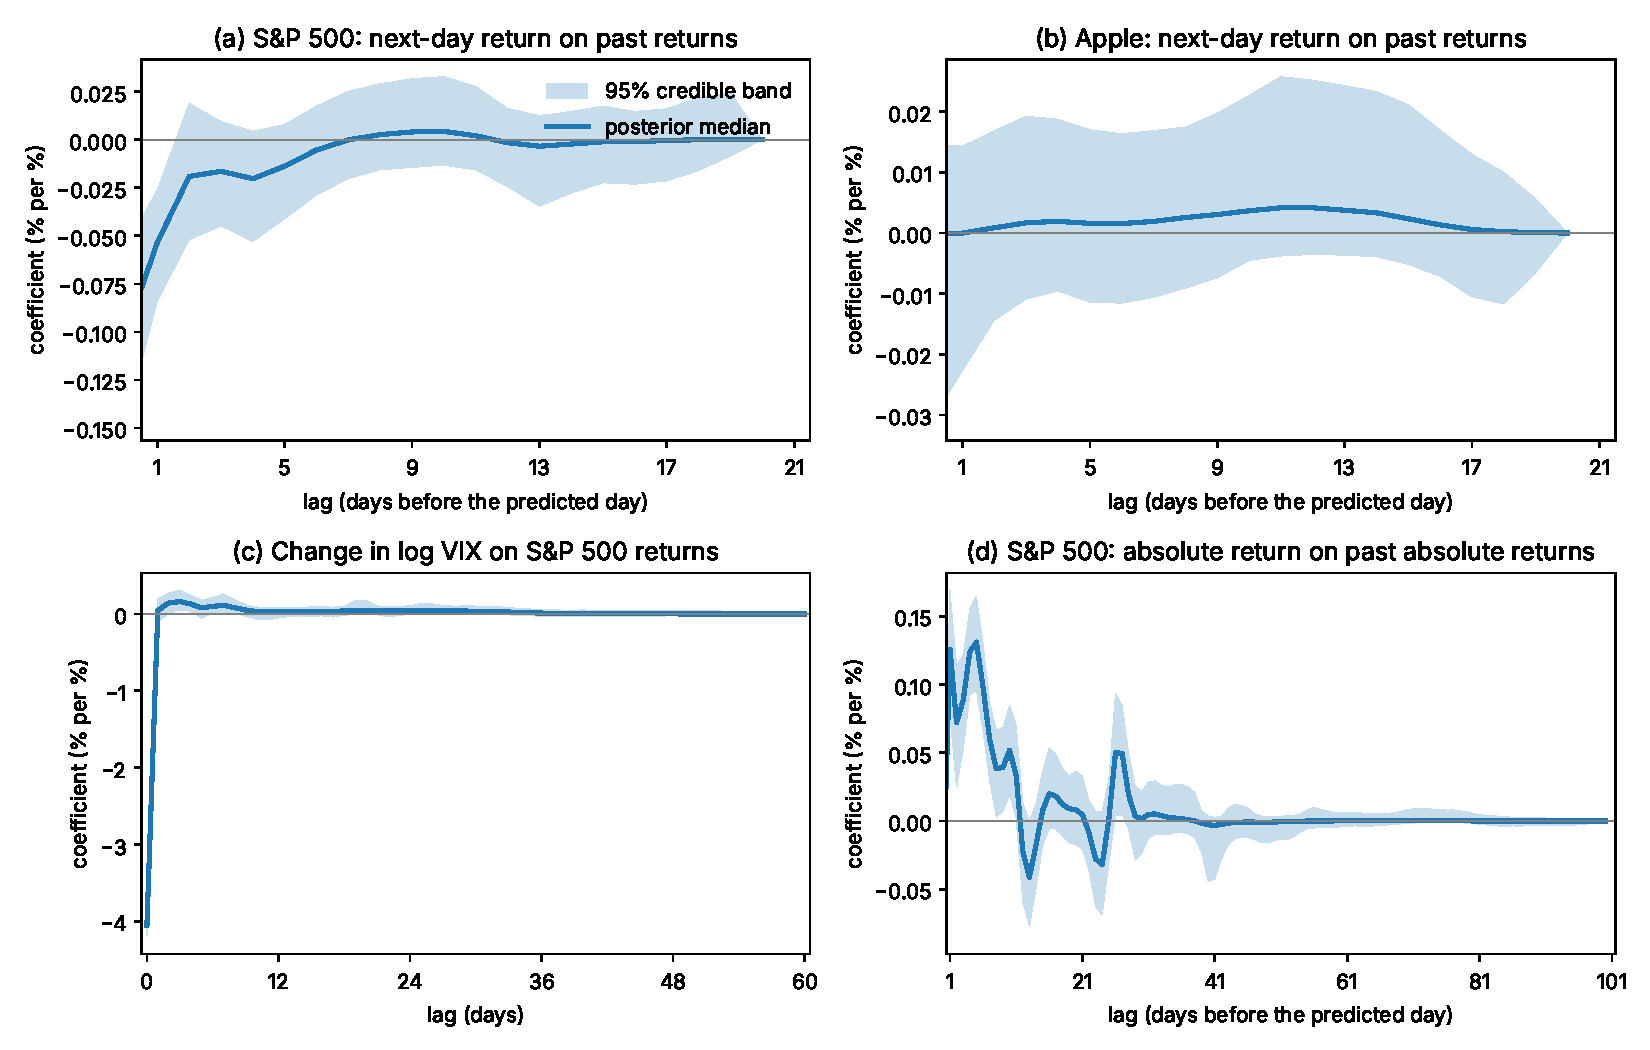
\includegraphics[width=\textwidth]{figures/stocks_lag_curves.pdf}
\caption{Lag curves for daily stock market data, 2007 to 2016: posterior
medians with 95\% credible bands. (a) Next-day S\&P 500 return on the previous
20 days' returns; (b) the same for Apple; (c) daily change in log VIX on
contemporaneous and lagged S\&P 500 returns; (d) log absolute S\&P 500 return
on its own past over 100 days.}
\label{fig:stocks}
\end{figure}

\subsection{Air pollution and mortality in Chicago}

The setting that motivated much of the distributed lag literature is the
delayed effect of air pollution on daily mortality, and in particular the
question of mortality displacement raised in Section \ref{sec:intro}. The
\texttt{chicagoNMMAPS} data distributed with the R package \texttt{dlnm}
\citep{gasparrini2011} contain daily counts of all-cause, cardiovascular and
respiratory deaths in Chicago from 1987 to 2000, 5,114 days with means of 115,
51 and 9 deaths per day, together with PM10 (mean 34 micrograms per cubic
metre, 5 per cent of days interpolated), temperature and dew point. Log deaths
were regressed on 40 lags of PM10 with the usual adjustments of this
literature as unpenalised terms: a B-spline of time with seven degrees of
freedom per year for trend and season, weekday indicators, and B-splines of
temperature and dew point, with AR(1) errors. Coefficients are expressed as the
percentage change in deaths per 10 micrograms per cubic metre.

Figure \ref{fig:chicago} shows the three lag curves and their cumulative
sums. For all-cause deaths the curve is positive on the day of exposure, 0.15
per cent (95\% interval $-0.02$ to $0.36$), falls through zero within three
days and is negative from about lag four to lag ten, where the band excludes
zero, before returning to zero. The cumulative effect over 40 days is
$-0.20$ per cent ($-1.30$ to $0.85$): deaths are brought forward by a few days
rather than added, the displacement pattern of \citet{schwartz2000} and
\citet{zanobetti2000}, and the lag curve exhibits it without any lag structure
having been specified in advance. The curve uses about five effective degrees
of freedom. Cardiovascular deaths show the same shape with smaller amplitude,
and respiratory deaths, at nine per day, are too few to show anything beyond
a wide band around zero.

\begin{figure}[t]
\centering
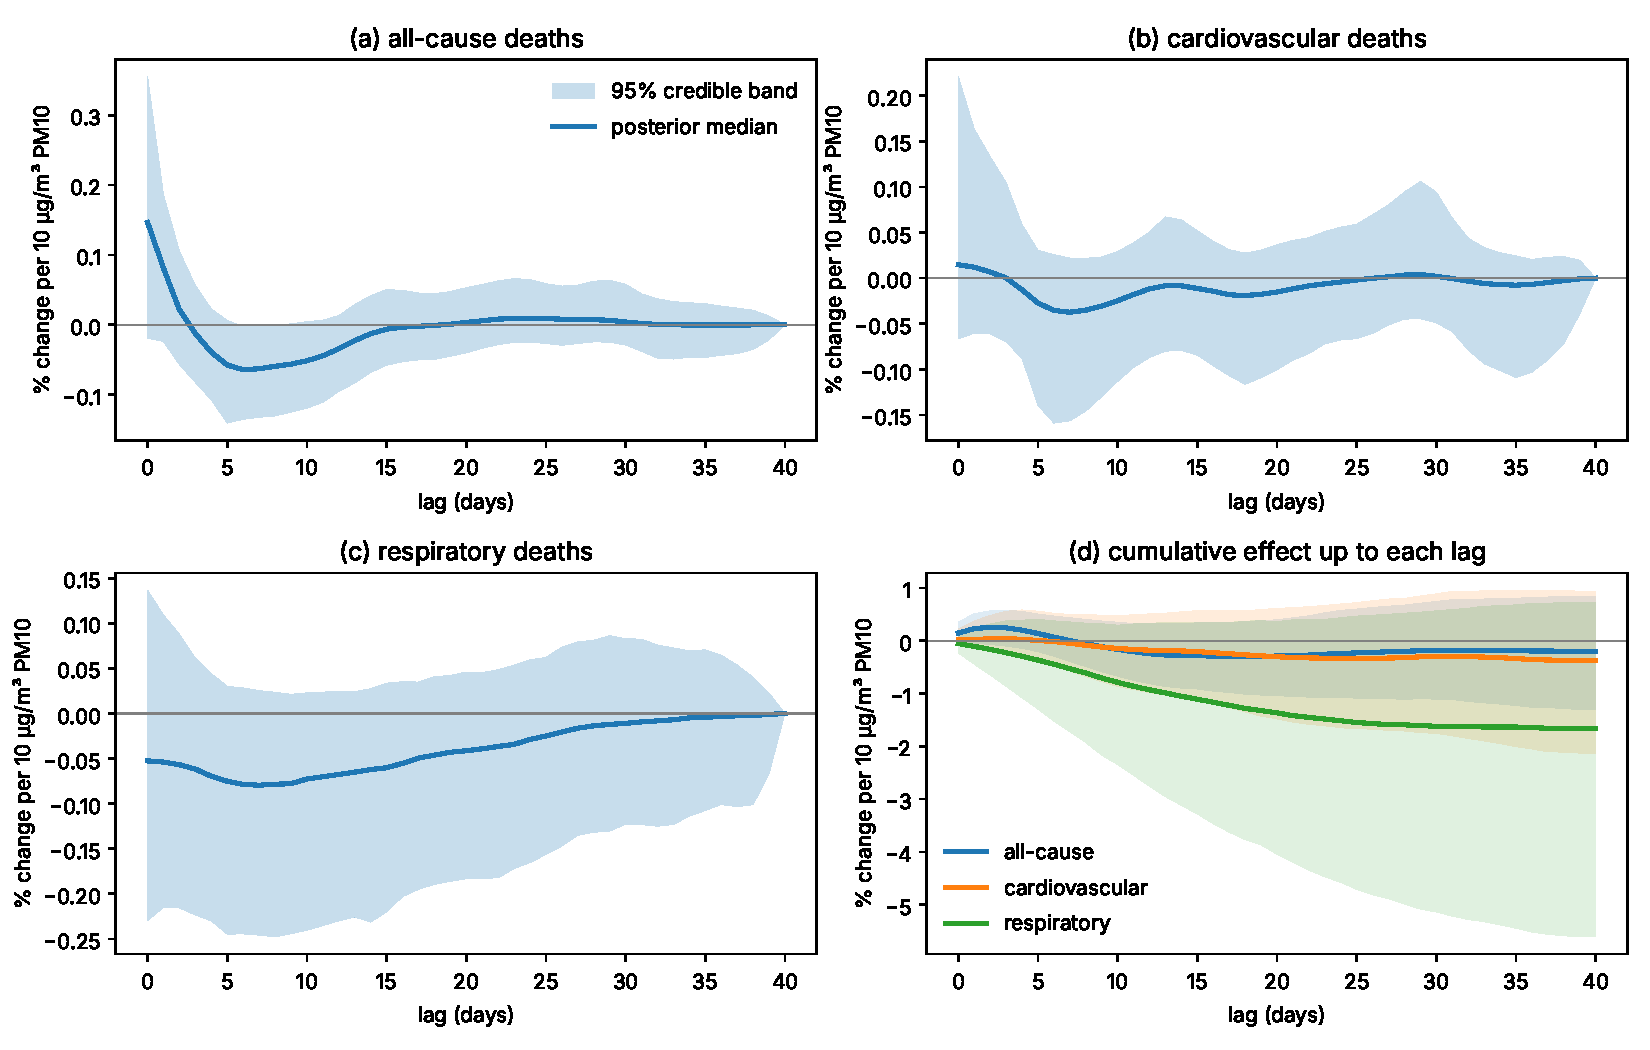
\includegraphics[width=\textwidth]{figures/chicago_lag_curves.pdf}
\caption{Chicago, 1987 to 2000: percentage change in daily deaths per 10
micrograms per cubic metre of PM10 at lags 0 to 40 for (a) all-cause, (b)
cardiovascular and (c) respiratory deaths, with 95\% bands, and (d) the
cumulative effect up to each lag.}
\label{fig:chicago}
\end{figure}

\subsection{COVID-19 cases and deaths}

Deaths from COVID-19 follow infections after a delay of a few weeks, so the
lag curve relating daily deaths to earlier cases estimates both the size of
the relationship and the shape of the delay. Daily counts for the United
States from June 2020 to March 2021, 304 days with a mean of 1,471 deaths per
day, were taken from the compilation by The New York Times; the period
precedes any effect of vaccination on the case fatality ratio. The exposure is
the log of the seven-day trailing mean of new cases and the response is log
deaths, so the lag coefficients are elasticities. Weekday indicators absorb
the day-of-week pattern in death reporting and the errors follow an AR(1)
process to allow for the remaining serial correlation. Figure \ref{fig:covid}
shows the data and the fitted curve with $p = 35$. The cumulative elasticity
is 0.74 (0.66 to 0.81): a 10 per cent rise in cases is followed by roughly a 7 per
cent rise in deaths, the shortfall from one reflecting the fall in the case
fatality ratio over the period. The curve rises to a peak at about three weeks
and returns to zero by five, using under three effective degrees of freedom,
but the individual lag coefficients are poorly identified, because the smoothed case series is highly collinear across lags:
the data determine the total and the timing, and the adaptive prior supplies
the smoothness. Deaths reported on Tuesday to Friday are about 2.5 times
those reported on a Sunday. A negative binomial model for the raw counts,
shown dashed in Figure \ref{fig:covid}, agrees on the total elasticity, 0.73
(0.68 to 0.77), and on the peak, but its sampler did not converge
satisfactorily, with many divergent transitions and $\hat{R}$ of 1.4: the
dependence between the curve and its smoothing parameters that the Gaussian
model integrates out remains present in a count model, and a collapsed or
approximately collapsed scheme for count responses is a topic for further
work.

\begin{figure}[t]
\centering
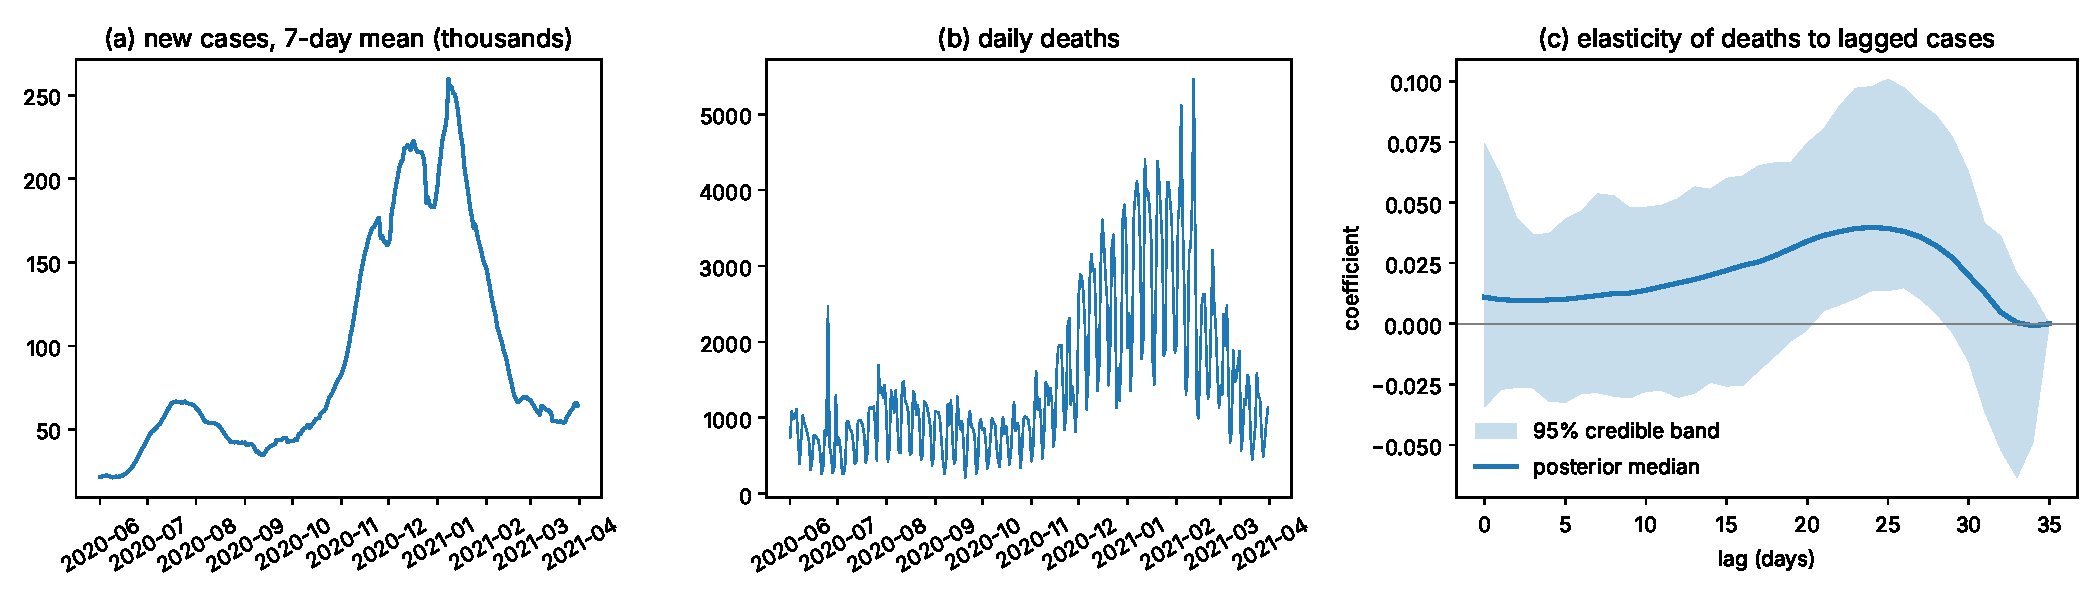
\includegraphics[width=\textwidth]{figures/covid_lag_curve.pdf}
\caption{COVID-19 in the United States, June 2020 to March 2021. (a)
Seven-day mean of new cases; (b) daily deaths; (c) elasticity of deaths to
cases at lags 0 to 35 under the Gaussian model for log deaths with AR(1)
errors (posterior median and 95\% band) and under a negative binomial model
for the counts (dashed).}
\label{fig:covid}
\end{figure}

\section{Discussion}
\label{sec:discussion}

This paper makes several important contributions. It was shown by simulation
in Section \ref{sec:sim} that estimation of lag structure can strongly depend
on the type of smoothing model that is assumed. Several existing DLM models
were shown to be non-robust to the choice of maximum lag $p$, even when the
underlying lag function is identical, which suggests that the interpretation
of lag estimates should be made with caution. A new model has been proposed
that combines automatic adaptive smoothing with a pragmatically large choice
of $p$ to ensure simple and flexible smoothing of the lag curve that avoids
sensitivity to the choice of $p$. The real data illustrations in Section
\ref{sec:real} show the adaptive curve reporting no structure where the data
contain none, a sharp and short-lived response where there is one, and a
slowly decaying response over a hundred lags, in each case with far fewer
effective parameters than the number of lags. The new approach provides users
of DLMs with a new way to explore their data with confidence that the
estimates are not contaminated by artefacts that result from particular model
choices.

\bibliographystyle{plainnat}
\bibliography{badlm}

\end{document}
